\addcontentsline{toc}{chapter}{Messdaten} % damit trotzdem im Inhaltsverzeichnis
\label{Protokoll}


% \thispagestyle{empty}

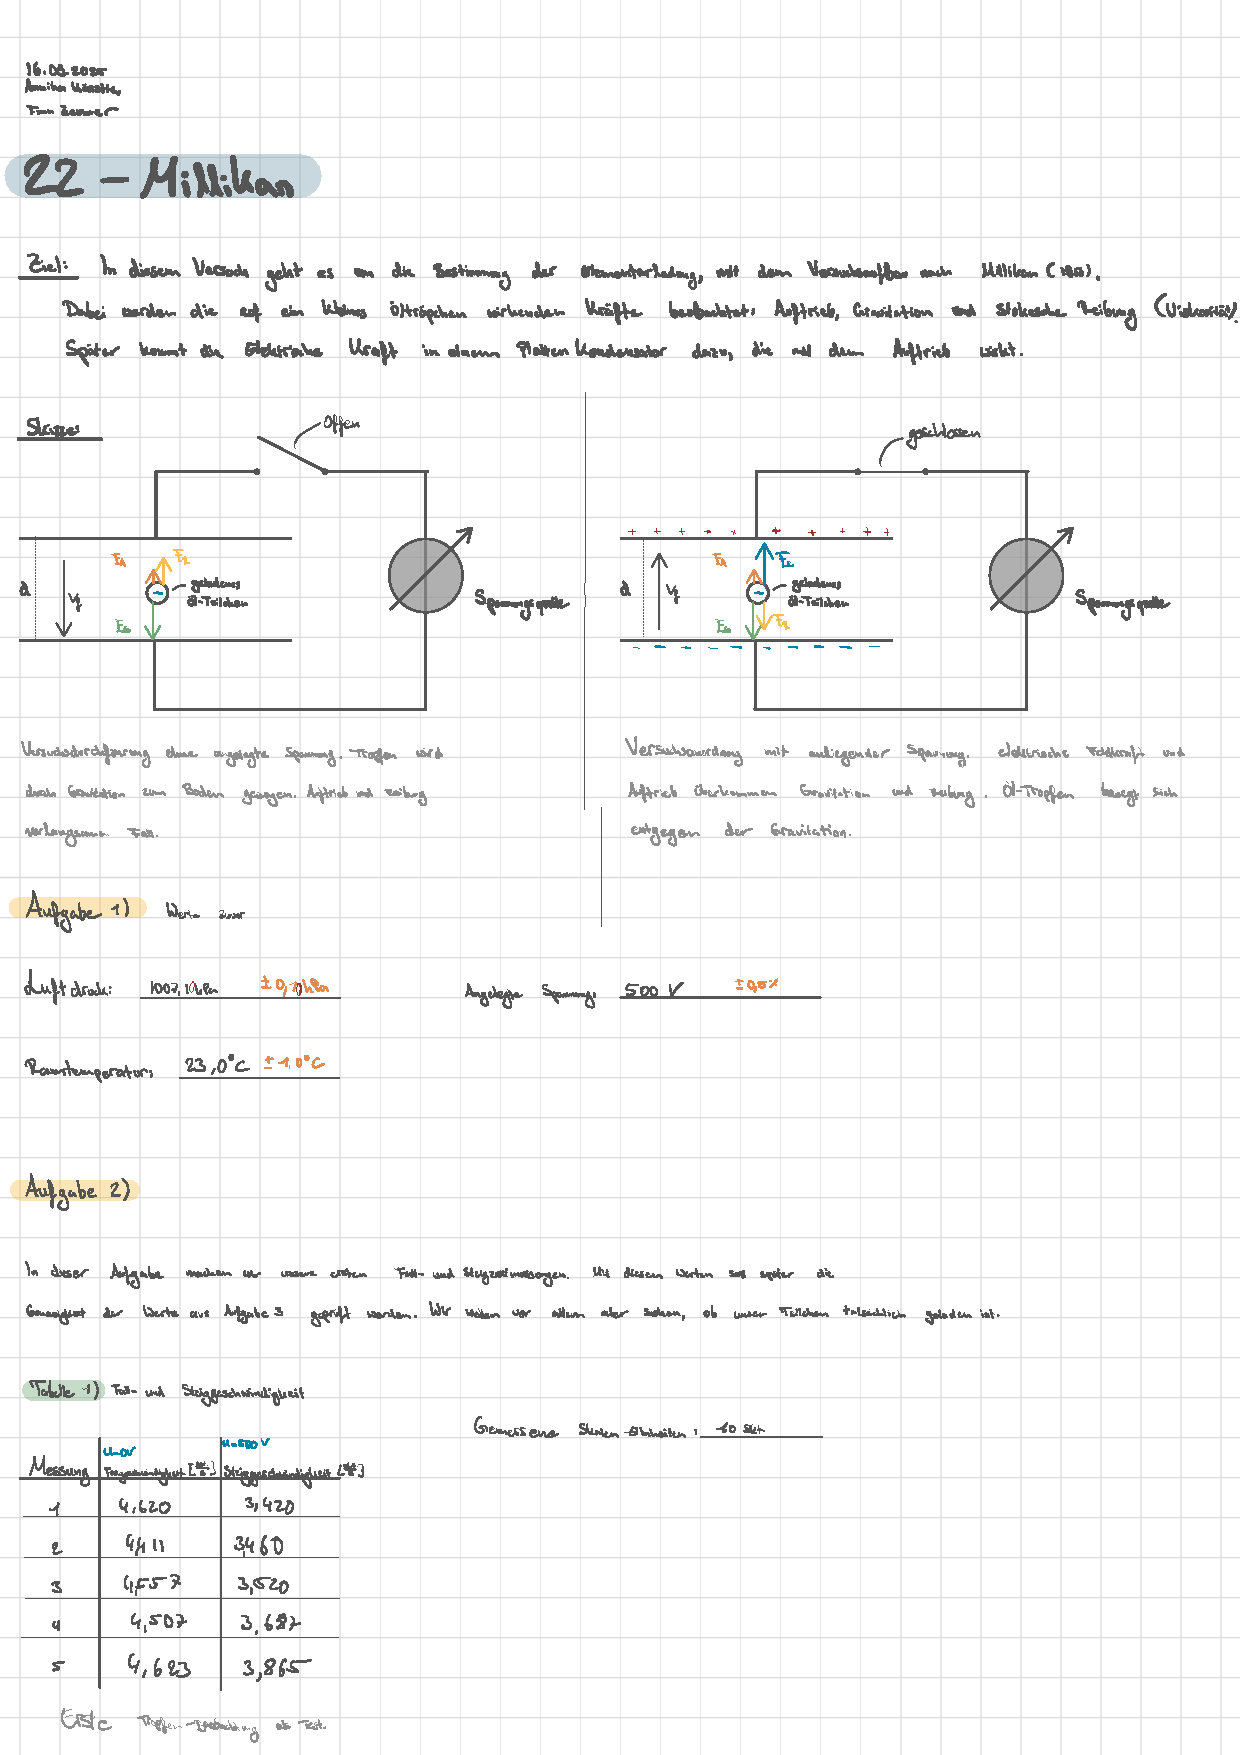
\includepdf[
  pages=-,               
  pagecommand={\thispagestyle{empty}} 
]{Protokolle/\versuchsnummer/Chapter/Messprotokoll.pdf}



\addcontentsline{lot}{table}{\protect\numberline{\thechapter.1} Messung der Wasserpegelhöhe für die Resonanz in der Luft}
\addcontentsline{lot}{table}{\protect\numberline{\thechapter.2} Messung der Wasserpegelhöhe für die Resonanz in der CO$_2$}
\addcontentsline{lot}{table}{\protect\numberline{\thechapter.2} Mikrophon-Lautsprecher-Abstand (Yt)}
\addcontentsline{lot}{table}{\protect\numberline{\thechapter.2} Mikrophon-Lautsprecher-Abstand (YX)}

\addcontentsline{lof}{figure}{\protect\numberline{\thechapter.1} Aufbau des Quincke'schen Rohrs}
\addcontentsline{lof}{figure}{\protect\numberline{\thechapter.2} Stehende Welle}
\addcontentsline{lof}{figure}{\protect\numberline{\thechapter.3} Resonanz im Quincke'schen Rohr}
\addcontentsline{lof}{figure}{\protect\numberline{\thechapter.3} Versuchsaufbau Oszilloskop}
